\chapter{A Tight Bound on Grids of Size $\geq$ 7}

\section{Introduction and Definitions}
Let the ordered tuple $(a,b,c)$ represent the $a \times b \times c$ grid $G$ where $a \geq b \geq c$. We refer to $c$ as the ``thickness" of $G$. For example, the tuple $(5,3,3)$ represents a $5 \times 3 \times 3$ grid of thickness 3. We refer to a tuple as ``divisible", or a ``divisibility case", if and only if $ab+bc+ca \equiv 0 \pmod 3$. Observe that the divisibility cases are precisely those grids with integral lower bounds. The divisibility cases of thicknesses belonging to the three residue classes modulo 3 are illustrated in \{Figure something\}.

In the following lemmas, we use the notation $(a,b,c)+(x,y,z) = (a+x, b+y, c+z)$ to represent respective increases of $x$, $y$, and $z$ to the side lengths $a$, $b$, and $c$ of $G$. We note the following: 
\begin{rem}
By applying the recursion, $(a,b,c)+(x,y,z)$ percolates at the lower bound when either:
\begin{enumerate}
\item $(a,b,c), (a,y,z), (x,b,z), (x,y,c)$ all percolate at the lower bound, or;
\item $(x,y,z), (x,b,c), (a,y,c), (a,b,z)$ all percolate at the lower bound.
\end{enumerate}
\end{rem}

We shall call a thickness ``complete" if it can be shown that all divisibility cases in that thickness percolate at the lower bound. In this section, we demonstrate that thickness 5, thickness 6 and thickness 7 are all complete. As these belong to the residue classes 2, 0, and 1 modulo 3, respectively, we then use a recursive construction to show that all larger grids are also complete. 

\section{Completeness of Thickness 5}
Leveraging \{lemmas from earlier chapters yet to be written\}, we show that all divisibility cases in thickness 5 percolate at the lower bound. 

\begin{lem}
Thickness 5 is complete.
\end{lem}

\begin{proof}
Let $(a,b,2)$ represent an arbitrary (divisible) grid of thickness 2, and let $x = a \pmod 6$ and $y = b \pmod 6$. By \{some as of yet unwritten construction\}, we have that $(a,b,2)$ percolates at the lower bound for all $x,y \in \{0,2,3,5\}$, where $x \neq y$. We consider two constructions: $(a,b,2) + (6,3,3)$ and $(a,b,2) + (6,6,3)$. 

By item (1) of the remark, in order to show that $(a,b,2) + (6,3,3)$ percolates at the lower bound, it is sufficient to show that $(a,b,2), (a,3,3), (6,b,3), (6,3,2)$ all percolate at the bound. By \{more unwritten constructions\}, this is true for all $x,y \in \{0,2,3,5\}$, where $x \neq y$ and at least one of $\{a,b\} > 2$. (Note that if $a=2$, one of the tuples is $(2,3,3)$, which does not percolate at the lower bound; we accommodate for this by re-writing $(a,b,2) + (6,3,3)$ as $(a,b,2) + (3,6,3)$.) The resulting tuple $(a', b', 5)$ is a grid of thickness 5, with $a'$ and $b'$ in the same residue class modulo $6$, and at least one of $\{a',b'\} \geq 9$. From \{some figure representing the divisibility cases of thickness 5\}, we see that the lower bound on $a'$ and $b'$ omits the following three grids: $(5,5,5), (6,6,5)$ and $(8,8,5)$. 

Applying an analogous argument to $(a,b,2) + (6,6,3)$, we must demonstrate that $(a,b,2), (a,6,3), (6,b,3), (6,6,2)$ all percolate at the lower bound. By \{some other constructions\}, we again find that this holds for all $x,y \in \{0,2,3,5\}$, where $x \neq y$ and $a,b > 1$. This gives all thickness 5 tuples $(a',b', 5)$ with $a'$ and $b'$ in different residue classes modulo $6$, where $a',b' \geq 8$. 

SOMETHING IS DIFFERENT

\begin{figure}[]
\centering
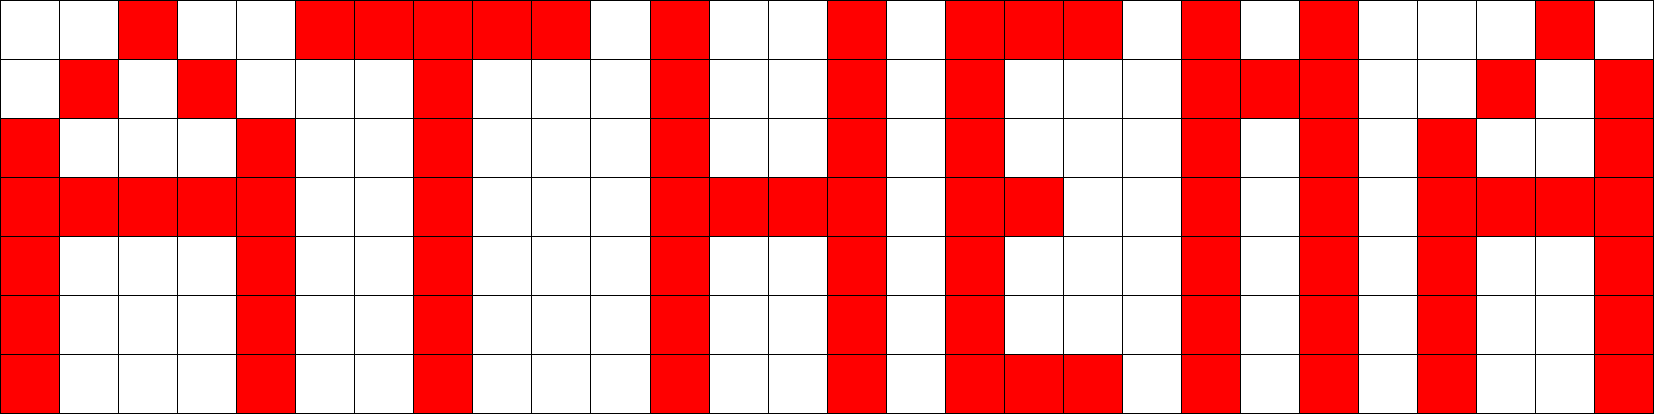
\includegraphics[height=1in]{figures/3/7x28x1.pdf}
\end{figure}

\end{proof}

\subsection{Intuition and Statement}

\subsection{Proof}